\documentclass[11pt]{article}
\usepackage[utf8]{inputenc}
\usepackage[parfill]{parskip}
\usepackage{graphicx}
\usepackage{enumerate}
\usepackage{amsmath}
\usepackage[title]{appendix}
\usepackage[margin=25mm]{geometry}
\usepackage{amsmath,graphicx,psfrag,pstricks}
\def\n{\noindent}
\def\u{\underline}
\usepackage{gensymb}
\def\hs{\hspace}
\newcommand{\thrfor}{.^{\displaystyle .} .}
\newcommand{\bvec}[1]{{\bf #1}}
\usepackage{graphicx}
\usepackage{rotating}
\graphicspath{{Plots/}}
\usepackage{amsmath}
\usepackage{booktabs}
\usepackage{siunitx}
\usepackage{amssymb}
\usepackage[utf8]{inputenc}
\usepackage[justification=centering]{caption}
\usepackage{float}
\usepackage{listings}
\usepackage{color} %red, green, blue, yellow, cyan, magenta, black, white
\definecolor{mygreen}{RGB}{28,172,0} % color values Red, Green, Blue
\definecolor{mylilas}{RGB}{170,55,241}
\lstset{language=Matlab,%
    %basicstyle=\color{red},
    breaklines=true,%
    morekeywords={matlab2tikz},
    keywordstyle=\color{blue},%
    morekeywords=[2]{1}, keywordstyle=[2]{\color{black}},
    identifierstyle=\color{black},%
    stringstyle=\color{mylilas},
    commentstyle=\color{mygreen},%
    showstringspaces=false,%without this there will be a symbol in the places where there is a space
    numbers=left,%
    numberstyle={\tiny \color{black}},% size of the numbers
    numbersep=9pt, % this defines how far the numbers are from the text
    emph=[1]{for,end,break},emphstyle=[1]\color{red}, %some words to emphasise
    %emph=[2]{word1,word2}, emphstyle=[2]{style},  
}
\title{Part IIA Project - SF1: Data Analysis - Second Interim Report}
\author{Bailey Brookes | Corpus Christi | bdb31}
\date{\today}

\begin{document}
\maketitle

\section{\texttt{overlap\_add.m}}
Below are answers to the questions posed in the handout about the \texttt{overlap\_add.m} file.
\begin{enumerate}[(a)]
	\item This script is a simple attempt at the Wiener filter but with constant filter gains of 0.1 and 0.2. Also, this filter use the overlap add technique. 
	\item Weiner filters can be implemented in time or frequency domain. The multiplication of gains in frequency is the same as convolving them in time, meaning filtering in frequency or time produces the same results.
	\item Direct convolution filtering has complexity of $O(N^2)$ while FFT convolution has complexity of $O(N\log N)$. When the number of samples, N, per frame is 516 this means FFT convolution is:
		\[
	\frac{N^2}{N\log N} = \frac{516^2}{516\log 516} \approx 57.3 \hspace{0.2cm}\text{faster}
	\]
	\item \texttt{conj} takes the complex conjugate of a complex number so as the FFT is symmetric, only one half needs to be filters (0 to $\pi$) and then the second half ($\pi$ to $2\pi$) is the complexity conjugate of the first half.
\end{enumerate}

\section{Noise Reduction}
\subsection{Basic de-noising: \texttt{bdb31\_noiseReduction.m}}
\texttt{bdb31\_noiseReduction.m} is the script that de-noises the required 4 audio files using a basic overlap add Weiner filter. It predicts the power spectrum of the noise using the initial silent portion of the audio, and zero pads each frame to increase precision without adding too much run time. Zero padding reduces the digital distortion resulting from filter gains of zero, which result in sharp jumps in the time domain which is head as digital noise.he resulting filtered audio is good, with minimal digital noise and almost all the random noise from the file removed. 

The mean squared error (MSE) is calculated and presented after each run. The MSE however doesn't fully convey the quality of the filtered audio. For example, before zero padding there is a lot of digital distortion but the MSE result is very small, even though the audio is of a very poor quality. Furthermore, smoothing the signal using Matlab \texttt{smooth} also decreases the MSE but the audio becomes considerably quieter and 'merky', like it's being heard through a wall. Hence, zero padding is used without smoothing.

In deciding the parameters, changing the frame length has an interesting effect on the MSE, as show in Figure BLANK. MSE is almost periodic and overall lower at shorter frame lengths. However to smaller frame length result in audible distortion so a trade off is need. For my filter, a frame length of 256 and overlap 128 is used  a hann. window

\subsubsection{Time varying noise}
For the two time varying noise files, the basic Weiner filter works well. This is because the power spectrum of the noise is calculated from the variance of the initial silent bit of the audio, which takes into the account the changing noise level. This is very basic and a better filter would calculate the power spectrum of the noise for each frame and use that for the filter coefficients for each frame.

\subsection{De-noising files without a silent portion: \texttt{bdb31\_noSilenceReduction.m}}
Some files, such as \texttt{Fast\_N.wav} don't have a silent portion from which the variance of the noise can be estimated. A different method therefore must be used.

One method is to smooth the original data and then subtract this smoothed data from the original data to get an estimate of the noise. This is done for each individual frame and produces a file with the noise removed but more digital noise is added than in the simple de-noising case that estimates the noise level using the silent portion.

\subsubsection{Time-varying noise}
The time varying noise files where also filtered using this method for comparison with the silent estimate case. While this method estimates the noise better, there is more digital distortion caused using the smoothed technique. Both are presented so methods can be compared.

\appendix

\section{How audio files where filtered}
The file are saved using the following naming convention so the filter used is clear:

{\centering
\texttt{orginal\_file\_name.wav\_filtered\_method.wav} \par}

Where \texttt{method} tells you how the noise was estimated either using the silent portion method, denoted \texttt{silent}, or smoothing each frame and subtracting the smoothed version from the original to estimate the noise, denoted \texttt{smooth}.

\section{Plots}

\begin{figure} [H]
\centering	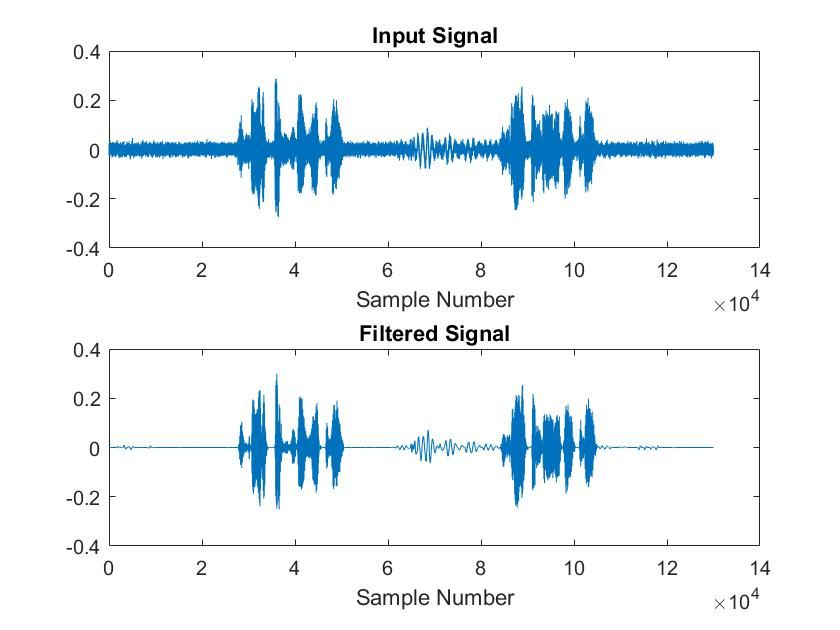
\includegraphics[scale = 0.4]
{male_loud_filter}
\caption{Plot of Input and filtered signal of male\_speech\_noisy\_loud.wav. The script also produces plots for all files it filters.}
\label{man_soft}
\end{figure}

\begin{figure} [H]
\centering	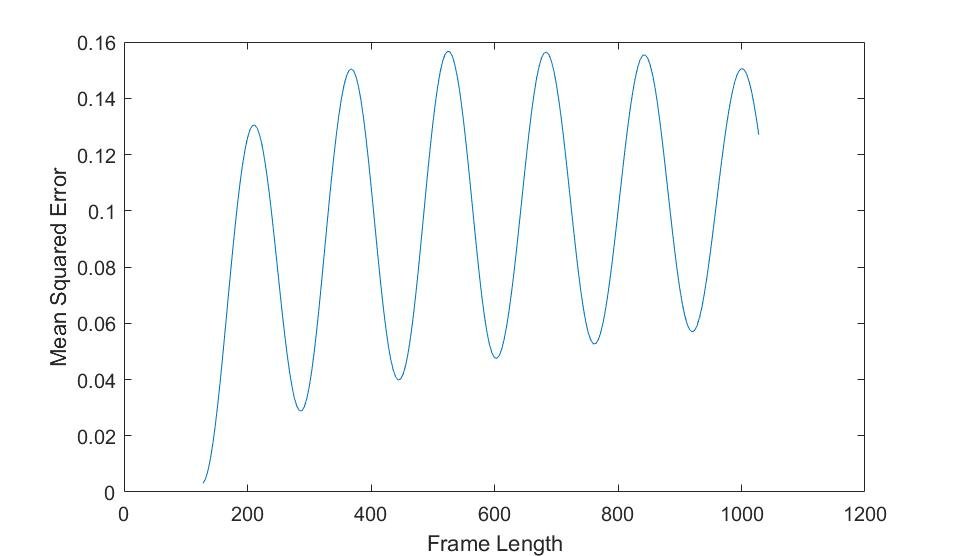
\includegraphics[scale = 0.4]
{MSE_Framelength}
\caption{Plot of Mean squared error vs frame length for the overlap add Weiner filter}
\label{MSE}
\end{figure}

\end{document}